\paragraph{Verdict stability.}

On CALM, duplication changes 22.6\% of 4B brief-prompt verdicts (146 of 646 ordered comparisons, 95\% interval 19.7 to 25.5\%). The 0.6B model selects an answer on just 0.2\% of unedited comparisons under the brief prompt. Unchanged-input repeats reproduce 1,200 of 1,200 CALM verdicts. Table~\ref{tab:extension-calm} gives the flip rates for each style and prompt.

\begin{table}[t]
\centering
\small
\setlength{\tabcolsep}{4.5pt}
\begin{tabular}{@{}lrrr@{}}
\toprule
Judge and prompt & Verb. & Conf. & Fmt. \\
\midrule
0.6B brief & 0.5 & 0.2 & 0.2 \\
0.6B rubric & 0.3 & 0.2 & 0.0 \\
1.7B brief & 6.3 & 4.2 & 3.9 \\
1.7B rubric & 4.8 & 2.3 & 1.5 \\
4B brief & 22.6 & 5.3 & 4.0 \\
4B rubric & 19.3 & 9.8 & 5.3 \\
\bottomrule
\end{tabular}
\caption{Same-order flip rates in percent across 323 CALM pairs using A/B/tie scoring.}
\label{tab:extension-calm}
\end{table}

\paragraph{Accuracy and error transitions.}

Under the brief prompt, Qwen3-4B's accuracy is 53.65\% on the originals, 53.72\% when the correct answer is duplicated, 53.14\% when the incorrect answer is duplicated, and 54.17\% when both are duplicated. Incorrect-answer duplication yields a 0.51-point loss (95\% interval for loss -2.2 to 3.2 points). Among 499 originally correct ordered decisions, 94 changed to the incorrect answer and 1 changed to a tie. These are raw counts across pairs and orders. The estimates and intervals weight each source question equally.

Table~\ref{tab:extension-verbosity} compares duplication across all models and prompts. Figure~\ref{fig:extension-style} shows the direction and size of all three edits when applied to either answer.

\begin{figure*}[t]
\centering
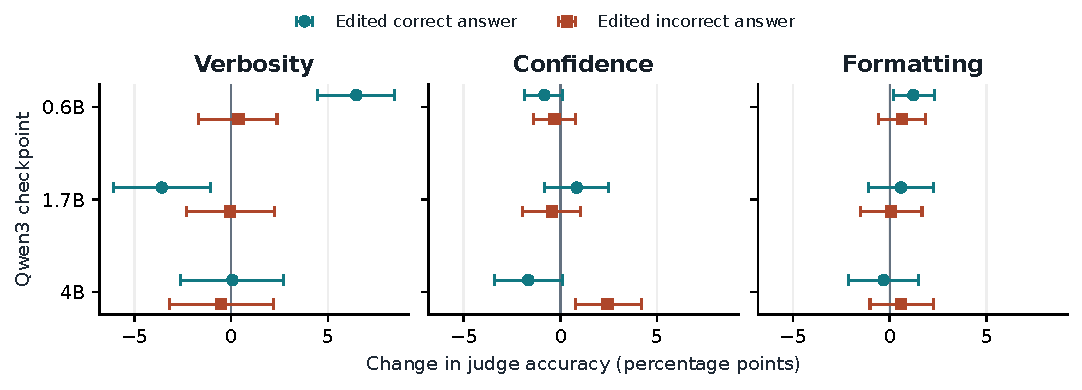
\includegraphics[width=.96\textwidth]{extension_generated/accuracy_changes.pdf}
\caption{Change in JudgeBench accuracy under the brief prompt and ordered A/B/tie scoring. Each point compares an edited condition with its original on the same questions. Whiskers are paired, question-clustered 95\% bootstrap intervals.}
\label{fig:extension-style}
\end{figure*}

\begin{table}[t]
\centering
\small
\setlength{\tabcolsep}{4.5pt}
\begin{tabular}{@{}lrrrr@{}}
\toprule
Judge and prompt & Orig. & Right & Wrong & Both \\
\midrule
0.6B brief & 23.4 & 29.9 & 23.8 & 30.7 \\
0.6B rubric & 12.6 & 14.6 & 11.9 & 13.9 \\
1.7B brief & 49.2 & 45.6 & 49.1 & 45.8 \\
1.7B rubric & 49.2 & 49.6 & 49.3 & 50.8 \\
4B brief & 53.7 & 53.7 & 53.1 & 54.2 \\
4B rubric & 53.8 & 44.8 & 58.3 & 53.1 \\
\bottomrule
\end{tabular}
\caption{JudgeBench accuracy in percent with ordered A/B/tie scoring. Right, wrong, and both specify which original answers were duplicated. Accuracy includes ties as errors.}
\label{tab:extension-verbosity}
\end{table}

\paragraph{Rubric and pooling.}

For 4B, the estimated reduction in incorrect-duplication loss from using the rubric is +5.0 points (95\% interval 1.6 to 8.5). With the brief prompt, the estimated reduction from A/B/tie pooling is -1.7 points (95\% interval -6.4 to 3.2). Positive reductions favor the intervention. Table~\ref{tab:extension-mitigation} shows the accuracy level and coverage for each 4B method.

\begin{table}[t]
\centering
\small
\setlength{\tabcolsep}{4.5pt}
\begin{tabular}{@{}lrrr@{}}
\toprule
4B prompt and rule & Orig. & Wrong & Cov. \\
\midrule
Brief / Single order & 53.7 & 53.1 & 99.6 \\
Brief / Order pool & 58.6 & 56.4 & 99.7 \\
Brief / Single order, forced & 53.7 & 53.5 & 100.0 \\
Brief / Order pool, forced & 58.7 & 56.9 & 100.0 \\
Rubric / Single order & 53.8 & 58.3 & 98.1 \\
Rubric / Order pool & 55.0 & 69.5 & 98.3 \\
Rubric / Single order, forced & 54.9 & 59.8 & 100.0 \\
Rubric / Order pool, forced & 57.7 & 71.2 & 100.0 \\
\bottomrule
\end{tabular}
\caption{Accuracy and coverage in percent for Qwen3-4B. Wrong is accuracy with the incorrect answer duplicated. Cov. is the fraction choosing an answer in that condition. Forced choice scores the same stored logits with only two candidate labels.}
\label{tab:extension-mitigation}
\end{table}

\paragraph{Precision check.}

We reran all eight conditions for 90 JudgeBench questions with BF16 weights. Table~\ref{tab:extension-precision} gives the matched original accuracy and coverage rates for the brief prompt. The analysis files give all paired style shifts and both prompts. Input token hashes matched between precisions.

\begin{table}[t]
\centering
\small
\setlength{\tabcolsep}{4.5pt}
\begin{tabular}{@{}lrrrr@{}}
\toprule
Qwen3 & NF4 Acc. & BF16 Acc. & NF4 Cov. & BF16 Cov. \\
\midrule
0.6B & 25.0 & 41.1 & 47.2 & 80.0 \\
1.7B & 50.6 & 50.0 & 98.3 & 95.0 \\
4B & 55.6 & 53.3 & 100.0 & 98.3 \\
\bottomrule
\end{tabular}
\caption{Matched NF4 and BF16 results in percent on unedited labeled pairs with the brief prompt. Accuracy includes ties as errors. Coverage is the share selecting an answer.}
\label{tab:extension-precision}
\end{table}

\paragraph{Exploratory format screen.}

A stricter screen for explicit output formats leaves 343 labeled pairs. The primary contrast on this subset is +0.4 points of accuracy loss (95\% interval -2.7 to 3.6 points). We added this sensitivity check after inspecting cases. The primary sample stays fixed.
